\section{\label{III-A-2}Des labyrinthes d'identifiants: les hubs de liens}
\titreEntete{Les hubs de liens}

%intro
La modélisation des données sous la forme de labyrinthes --- ou de graphes --- a un impact  considérable dans le Web de données: certains jeux de données sont eux-mêmes stockés dans une base de données graphe --- comme Wikidata qui fonctionne sur la base de données Blazegraph---; ou alors les jeux de données peuvent entre eux former un gigantesque graphe, infini. Cette seconde conception du modèle-réseau de \nP{Umberto}{Eco} est au centre du Web de données. Avec la décentralisation des référentiels sur le Web et leur éclatement en de multiples données, il est apparu comme nécessaire de les recentraliser au travers de nouveaux référentiels fournisseurs d'un unique identifiant.\\

Cependant, la recentralisation passe également par l'ajout de données, parallèlement à l'ajout des liens. En effet, nous l'avons montré au \reference{II-C}: les données peuvent varier dans leur graphie et leur forme selon le référentiel duquel elles sont issues. Afin d'offrir des données utilisables par tous, certaines plateformes ajoutent, pour chacun de leurs identifiants, des données préférentielles aux côtés des liens pointant vers d'autres référentiels ou jeux de données.

\subsection{\label{III-A-2-a}De la décentralisation des référentiels à leur recentralisation dans le Web de données}
\titreEntete{De la décentralisation des référentiels à leur recentralisation}

La multiplication du nombre de référentiels dans le Web de données conduit à une profusion de données et à leur répétition, sans que soient repérées les données se rapportant à un même concept\footnote{La constellation du Linked Open Data montre cette augmentation croissante du nombre de référentiels dans le Web de données, et l'absence, pour certains, de liens vers d'autres référentiels. Voir \reference{annexe_lod} (\reference{lod_cloud}).}. L'importance prise par ces référentiels partagés, mis en commun, et réutilisés par tous, a provoqué une recentralisation autour de nouveaux référentiels, nés de l'agrégation d'autres de ces référentiels.\\

Étonnante au premier abord puisqu'elle reconstruit des jeux de données alors que le mouvement inverse a été initié avec le Web de données pour plus d'efficacité, cette réaction s'explique par la nécessité de créer davantage de liens entre les données et les référentiels\footnote{\og Ironie de l’histoire, alors que le Linked Open Data souhaitait mettre en relation des données hétérogènes et décentralisées chez différents fournisseurs, il aura suffi de 5 ans pour que les utilisateurs commencent à recentraliser leurs données au sein d’un espace unique\fg{} in \cite{poupeau_au-a_2018}}. Ces nouveaux référentiels constituent alors des \og hubs\fg{} centralisant et exposant les données et les liens selon les règles et les principes du Web de données. \index[ref]{lod@Linked Open Data (LOD)!wikidata@Wikidata}Wikidata a ici un rôle majeur et prouve qu'une base de connaissances unique et centralisée est essentielle.\\

Si Wikidata est une base ouverte, des enjeux commerciaux peuvent également s'emparer de cette problématique de la structure des données sur le Web et de la description des documents nativement numériques: Google créé ainsi une base de connaissances parallèle --- le Knowledge Graph ---, elle aussi sous la forme d'un graphe mais n'utilisant pas \ac{rdf}, utilisant Wikidata comme une source de données. De même qu'un langage universel était nécessaire pour décrire les documents sur le Web, un langage est nécessaire pour décrire les sites Web et leur offrir en échange un meilleur référencement: la puissance de Google, associé à Yahoo et Microsoft, lui permet ainsi d'imposer l'ontologie \index[ref]{relier@Relier!schema@schema.org}\href{https://www.schema.org}{schema.org} comme standard du Web pour la description des sites\footcite{poupeau_au-a_2018}, rejetant \index[ref]{echanges@Échanges!formats@Formats!rdf@RDF}\ac{rdf}a au profit de \ac{json}-LD\footnote{Une sérialisation en \ac{json} adaptée aux données liées. Voir \url{https://www.w3.org/TR/json-ld/}.}.\\

Le Knowledge Graph et l'ontologie schema.org sont les meilleurs exemples de l'utilisation idéale du Web de données et du Web sémantique. Ils ont été créés spécialement pour centraliser les données et y accéder par le seul langage machine. \index[ref]{lod@Linked Open Data (LOD)!wikidata@Wikidata}Wikidata, qui apparaît comme le référentiel le plus élevé dans le milieu bibliothéconomique\footnote{Voir \reference{III-A-2-c}.}, n'est plus qu'une source de données structurées pour les robots des moteurs de recherche utilisant \index[ref]{relier@Relier!schema@schema.org}schema.org. Le référentiel a désormais acquis la place principale, centrale, dans l'administration de données et leur recherche.

\subsection{\label{III-A-2-b}Apparition des hubs de liens et d'identifiants}
\titreEntete{Apparition des hubs de liens et d'identifiants}

De même que les ontologies apportent une couche supplémentaire aux données, en les liant entre elles malgré leurs différences, des hubs se forment pour centraliser les identifiants de différents référentiels afin d'avoir un unique lieu où y seront puisés d'autres identifiants: c'est le principe de l'interopérabilité par suivi de liens. Ces nouveaux hubs se trouvant dans le Web de données, il est normal et indispensable qu'ils se créent sur les principes et les formats qui le composent. Ainsi, ces hubs forment des concepts, ou des entités, qui rassemblent les liens de vedettes et de concepts identiques. Ces nouveaux concepts sont également désignés par des URIs servant d'identifiant pour chacun d'eux.\\

Ces hubs prennent une place centrale dans le Web de données et deviennent indispensables. Seulement, il peut être risqué de ne conserver, dans un système documentaire, qu'un seul identifiant, celui de ce hub. En effet, aucun de ces identifiants ou de ces liens --- y compris les identifiants \textit{ark:} de la Bibliothèque nationale de France (BnF) --- ne peuvent être considérés comme pérennes et sûrs. Au-delà des identifiants qui disparaissent sur le Web, les données qui leur sont associées sont supprimées\footnote{\og De très nombreuses initiatives d’exposition des données ont aujourd’hui disparu, emmenant avec elles non seulement les identifiants mais aussi les données elles-mêmes\fg{} in \cite{poupeau_au-a_2018}}. Certes, l'ampleur de Wikidata peut laisser penser que les entités et leurs identifiants seront disponibles à long terme, mais des aléas techniques, financiers ou politiques peuvent très bien conduire à la fermeture de ce service et donc à la disparition de l'ensemble des données. Nous verrons par la suite (\reference{III-A-3}) que la récupération de quelques identifiants majeurs est nécessaire en plus de l'identifiant de Wikidata, afin d'avoir à la fois un accès direct à ces identifiants --- sans suivre les liens --- et une relative sécurité quant à la conservation d'un lien avec un référentiel externe.\\

\begin{figure}[h!]
	\centering
	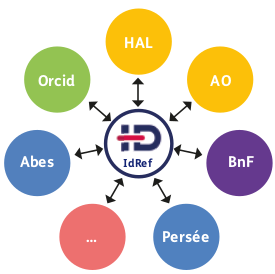
\includegraphics[width=7cm]{images/idref.png}
	\caption[La fédération entreprise par \ac{idref}]{La fédération entreprise par \ac{idref} [Source: \cite[p.9]{aymonin_arabesques_2017}]}
	\label{idref_schema}
\end{figure}

\index[ref]{lod@Linked Open Data (LOD)!viaf@VIAF}\index[ref]{autorites@Autorités!viaf@VIAF}\ac{viaf}, \index[ref]{lod@Linked Open Data (LOD)!idref@IDREF}\index[ref]{autorites@Autorités!idref@IDREF}\ac{idref} ou \index[ref]{lod@Linked Open Data (LOD)!lcsh@LCSH}\index[ref]{autorites@Autorités!lcsh@LCSH}\ac{lcsh} sont quelques uns de ces hubs de liens qui fournissent en une seule page plusieurs identifiants. \ac{idref} est basé sur les autorités du Sudoc, mais a été créé pour effectuer l'interopérabilité entre les différents catalogues du milieu de la recherche à travers un référentiel commun\footnote{\og Il s’agissait de montrer la fonction de pivot des identifiants et les bénéfices d’un adossement des catalogues à un référentiel commun.\fg{} in \cite[p.9]{aymonin_arabesques_2017}}. Ainsi, de multiples référentiels sont liés avec \ac{idref} par leur identifiant~(\reference{idref_schema}): \index[ref]{lod@Linked Open Data (LOD)!rameau@RAMEAU}\index[ref]{autorites@Autorités!rameau@RAMEAU}\ac{rameau} est utilisé, de même que HAL pour les publications scientifiques ouvertes ou Persée; les identifiants \ac{viaf} et \ac{isni} sont également renseignés, \dots


\subsection{\label{III-A-2-c}Les hubs de liens et d'identifiants réceptacles de données}
\titreEntete{Les hubs de liens et d'identifiants réceptacles de données}

\begin{citationLongue}
	D’un hub de références, Wikidata tend à devenir un réceptacle des données elles-mêmes\footcite{poupeau_au-a_2018}.
\end{citationLongue}
\medskip

Le projet \index[ref]{lod@Linked Open Data (LOD)!wikidata@Wikidata}Wikidata est né en 2012 de la volonté de centraliser les informations des Wikipédias sous la forme de données structurées en déclarations. Ce modèle de données ressemble à \index[ref]{echanges@Échanges!formats@Formats!rdf@RDF}\ac{rdf}, mais reste différent en raison des informations supplémentaires apportées par le modèle Wikidata: l'ajout de références et de qualificatifs enrichit les données. Wikidata s'impose dans le Web de données par ses atouts: ses données, augmentées par une communauté imposante, sont disponibles immédiatement et ne dépendent pas des mises à jour --- comme cela était le cas avec \index[ref]{lod@Linked Open Data (LOD)!dbpedia@DBpédia}DBpédia ---; les données de Wikidata se requêtent avec \index[ref]{echanges@Échanges!protocoles@Protocoles!sparql@SPARQL}\ac{sparql}.\\

Premièrement, Wikidata est un hub d'identifiants, de liens. Ces identifiants font l'objet, sur les pages d'entités de Wikidata, d'une partie à part, à la fin de cette page. Ils sont néanmoins de simples déclarations propriété--valeur avec une possibilité d'ajouter des qualificatifs et des références\footnote{Un compte Twitter, qui a un identifiant et qui peut par conséquent faire l'objet d'une déclaration dans une entité de Wikidata, a, par exemple, comme qualificatif le nombre d'abonnés à une date donnée.}.
L'ensemble --- plusieurs centaines --- des propriétés d'identifiants est répertorié sur la page de liste de ces propriétés (\href{https://www.wikidata.org/wiki/Wikidata:List_of_properties/Wikidata_property_for_an_identifier}{Wikidata:List of properties/Wikidata property for an identifier}): les jeux de données et les référentiels étant de plus en plus nombreux sur le Web, ces propriétés permettent de typer et de décrire chaque relation avec un identifiant.\\

Deuxièmement, \index[ref]{lod@Linked Open Data (LOD)!wikidata@Wikidata}Wikidata est un réceptacle de données. En effet, en plus des identifiants, Wikidata propose des déclarations structurées biographiques ou générales sur l'entité. En cela, si \index[ref]{lod@Linked Open Data (LOD)!idref@IDREF}\index[ref]{autorites@Autorités!idref@IDREF}\ac{idref} et Wikidata semblaient être similaires avec l'offre de liens, ils diffèrent par cette structuration permanente des informations. Ainsi,  le concept \nP{Vincent}{Dedienne} de \ac{idref}\footnote{\nP{Vincent}{Dedienne} dans \ac{idref}: \url{https://www.idref.fr/196914183}\\\nP{Vincent}{Dedienne} dans Wikidata: \url{https://www.wikidata.org/wiki/Q18413745}} structure l'état civil et les dates, mais met le reste des informations en note: \og Comédien, auteur, acteur et humoriste français\fg{}. Wikidata apporte du sens grâce à la propriété P106 qui permet d'indiquer que la déclaration concerne l'\textit{occupation} de la personne, et d'offrir un lien vers l'entité de cette occupation.\\

Par la structuration de ses données et l'apport de multiples identifiants et liens vers d'autres jeux de données et référentiels, \index[ref]{lod@Linked Open Data (LOD)!wikidata@Wikidata}Wikidata devient un \textit{super} hub, se plaçant plus haut encore que ceux évoqués précédemment.

%conclu
\bigskip
\bigskip
L'agrégation de liens et d'identifiants est un enjeu essentiel de manière à n'effectuer des opérations d'alignement qu'une seule fois, et ainsi diminuer le coût de ces opérations. Ces agrégations nécessitant elles-mêmes des identifiants pour pouvoir exister sur le Web de données, des données structurées sont venues s'ajouter à la simple exposition de liens vers d'autres référentiels. Ainsi, Wikidata a montré son efficacité et se place aujourd'hui comme acteur principal d'agrégation de connaissances et de liens vers d'autres sources de données souvent plus spécialisées.